\documentclass[portrait,final,a0paper,fontscale=0.277]{baposter}

\usepackage{calc}
\usepackage{graphicx}
\usepackage{amsmath}
\usepackage{amssymb}
\usepackage{relsize}
\usepackage{multirow}
\usepackage{rotating}
\usepackage{bm}
\usepackage{enumitem}
\usepackage{url}
\usepackage{booktabs}
\usepackage{graphicx}
\usepackage{multicol}
\usepackage{tabularx}
% ...

%\usepackage{times}
%\usepackage{helvet}
%\usepackage{bookman}
\usepackage{palatino}

\newcommand{\captionfont}{\footnotesize}

\graphicspath{{images/}{../images/}}
\usetikzlibrary{calc}


\newcommand{\Matrix}[1]{\begin{bmatrix} #1 \end{bmatrix}}
\newcommand{\Vector}[1]{\begin{pmatrix} #1 \end{pmatrix}}

\newcommand*{\norm}[1]{\mathopen\| #1 \mathclose\|}% use instead of $\|x\|$
\newcommand*{\abs}[1]{\mathopen| #1 \mathclose|}% use instead of $\|x\|$
\newcommand*{\normLR}[1]{\left\| #1 \right\|}% use instead of $\|x\|$

\newcommand*{\SET}[1]  {\ensuremath{\mathcal{#1}}}
\newcommand*{\FUN}[1]  {\ensuremath{\mathcal{#1}}}
\newcommand*{\MAT}[1]  {\ensuremath{\boldsymbol{#1}}}
\newcommand*{\VEC}[1]  {\ensuremath{\boldsymbol{#1}}}
\newcommand*{\CONST}[1]{\ensuremath{\mathit{#1}}}

\DeclareMathOperator*{\argmax}{arg\,max}
\DeclareMathOperator*{\diag}{diag}
\DeclareMathOperator*{\argmin}{arg\,min}
\DeclareMathOperator*{\vectorize}{vec}
\DeclareMathOperator*{\reshape}{reshape}

%\font\dsfnt=dsrom12

\newcommand{\SNN}{\ensuremath{\mathbb N}}
\newcommand{\SRR}{\ensuremath{\mathbb R}}
\newcommand{\SZZ}{\ensuremath{\mathbb Z}}
%-----------------------------------------------------------------------------
% Matrices of the shape model
\renewcommand{\a}{\VEC\alpha}
\renewcommand{\v}{\VEC v}
\renewcommand{\l}{\VEC l}
\newcommand*{\m}{\VEC{\mu}}
\newcommand*{\M}{\MAT{M}}
\renewcommand*{\P}{\MAT{\Pi}}

%\newcommand{\J}{\SET J}
\newcommand{\J}{\SET{P}}
\newcommand{\Active}{\mathcal{A}}
\newcommand{\Selection}{\mathbf{S}}
\newcommand{\AllSelections}{\mathfrak{S}}
\newcommand{\Params}{\VEC\Theta}

%%%%%%%%%%%%%%%%%%%%%%%%%%%%%%%%%%%%%%%%%%%%%%%%%%%%%%%%%%%%%%%%%%%%%%%%%%%%%%%%
%%%% Some math symbols used in the text
%%%%%%%%%%%%%%%%%%%%%%%%%%%%%%%%%%%%%%%%%%%%%%%%%%%%%%%%%%%%%%%%%%%%%%%%%%%%%%%%

%%%%%%%%%%%%%%%%%%%%%%%%%%%%%%%%%%%%%%%%%%%%%%%%%%%%%%%%%%%%%%%%%%%%%%%%%%%%%%%%
% Multicol Settings
%%%%%%%%%%%%%%%%%%%%%%%%%%%%%%%%%%%%%%%%%%%%%%%%%%%%%%%%%%%%%%%%%%%%%%%%%%%%%%%%
\setlength{\columnsep}{1.5em}
\setlength{\columnseprule}{0mm}

%%%%%%%%%%%%%%%%%%%%%%%%%%%%%%%%%%%%%%%%%%%%%%%%%%%%%%%%%%%%%%%%%%%%%%%%%%%%%%%%
% Save space in lists. Use this after the opening of the list
%%%%%%%%%%%%%%%%%%%%%%%%%%%%%%%%%%%%%%%%%%%%%%%%%%%%%%%%%%%%%%%%%%%%%%%%%%%%%%%%
\newcommand{\compresslist}{%
\setlength{\itemsep}{1pt}%
\setlength{\parskip}{0pt}%
\setlength{\parsep}{0pt}%
}

%%%%%%%%%%%%%%%%%%%%%%%%%%%%%%%%%%%%%%%%%%%%%%%%%%%%%%%%%%%%%%%%%%%%%%%%%%%%%%
%%% Begin of Document
%%%%%%%%%%%%%%%%%%%%%%%%%%%%%%%%%%%%%%%%%%%%%%%%%%%%%%%%%%%%%%%%%%%%%%%%%%%%%%

\begin{document}

%%%%%%%%%%%%%%%%%%%%%%%%%%%%%%%%%%%%%%%%%%%%%%%%%%%%%%%%%%%%%%%%%%%%%%%%%%%%%%
%%% Here starts the poster
%%%---------------------------------------------------------------------------
%%% Format it to your taste with the options
%%%%%%%%%%%%%%%%%%%%%%%%%%%%%%%%%%%%%%%%%%%%%%%%%%%%%%%%%%%%%%%%%%%%%%%%%%%%%%
% Define some colors

\definecolor{lightorange}{rgb}{0.9,0.4,0}
\definecolor{lightestorange}{rgb}{1,0.8,0.5}
\definecolor{darkorange}{rgb}{0.2,0.1,0}

\hyphenation{resolution occlusions}
%%
\begin{poster}%
  % Poster Options
  {
  % Show grid to help with alignment
  grid=false,
  % Column spacing
  colspacing=1em,
  % Color style
  bgColorOne=white,
  bgColorTwo=white,
  borderColor=darkorange,
  headerColorOne=darkorange,
  headerColorTwo=lightorange,
  headerFontColor=white,
  boxColorOne=lightestorange,
  boxColorTwo=lightorange,
  % Format of textbox
  textborder=faded,
  % Format of text header
  eyecatcher=true,
  headerborder=closed,
  headerheight=0.1\textheight,
%  textfont=\sc, An example of changing the text font
  headershape=roundedright,
  headershade=shadelr,
  headerfont=\Large\bf\textsc, %Sans Serif
  textfont={\setlength{\parindent}{1.5em}},
  boxshade=plain,
%  background=shade-tb,
  background=plain,
  linewidth=2pt
  }
  % Eye Catcher
  {
\includegraphics[height=4em]{images/Aminer_logo_big.png}} 
  % Title
  {\bf\textsc{Temporal Summarization of Knowledge Evolutionary Trend}\vspace{0.5em}}
  % Authors
  {\textsc{ Yutao Zhang, Ningping Wang and Jie Tang }}
  % University logo
  {% The makebox allows the title to flow into the logo, this is a hack because of the L shaped logo.
    
\includegraphics[height=7.0em]{images/Tsinghua_University_Logo.png}
  }

%%%%%%%%%%%%%%%%%%%%%%%%%%%%%%%%%%%%%%%%%%%%%%%%%%%%%%%%%%%%%%%%%%%%%%%%%%%%%%
%%% Now define the boxes that make up the poster
%%%---------------------------------------------------------------------------
%%% Each box has a name and can be placed absolutely or relatively.
%%% The only inconvenience is that you can only specify a relative position 
%%% towards an already declared box. So if you have a box attached to the 
%%% bottom, one to the top and a third one which should be in between, you 
%%% have to specify the top and bottom boxes before you specify the middle 
%%% box.
%%%%%%%%%%%%%%%%%%%%%%%%%%%%%%%%%%%%%%%%%%%%%%%%%%%%%%%%%%%%%%%%%%%%%%%%%%%%%%
    %
    % A coloured circle useful as a bullet with an adjustably strong filling
    \newcommand{\colouredcircle}{%
      \tikz{\useasboundingbox (-0.2em,-0.32em) rectangle(0.2em,0.32em); \draw[draw=black,fill=lightblue,line width=0.03em] (0,0) circle(0.18em);}}
      
%%%%%%%%%%%%%%%%%%%%%%%%%%%%%%%%%%%%%%%%%%%%%%%%%%%%%%%%%%%%%%%%%%%%%%%%%%%%%%
\headerbox{Visualization}{name=results,column=1,span=2,row=0}{
  %%%%%%%%%%%%%%%%%%%%%%%%%%%%%%%%%%%%%%%%%%%%%%%%%%%%%%%%%%%%%%%%%%%%%%%%%%%%%%

\centering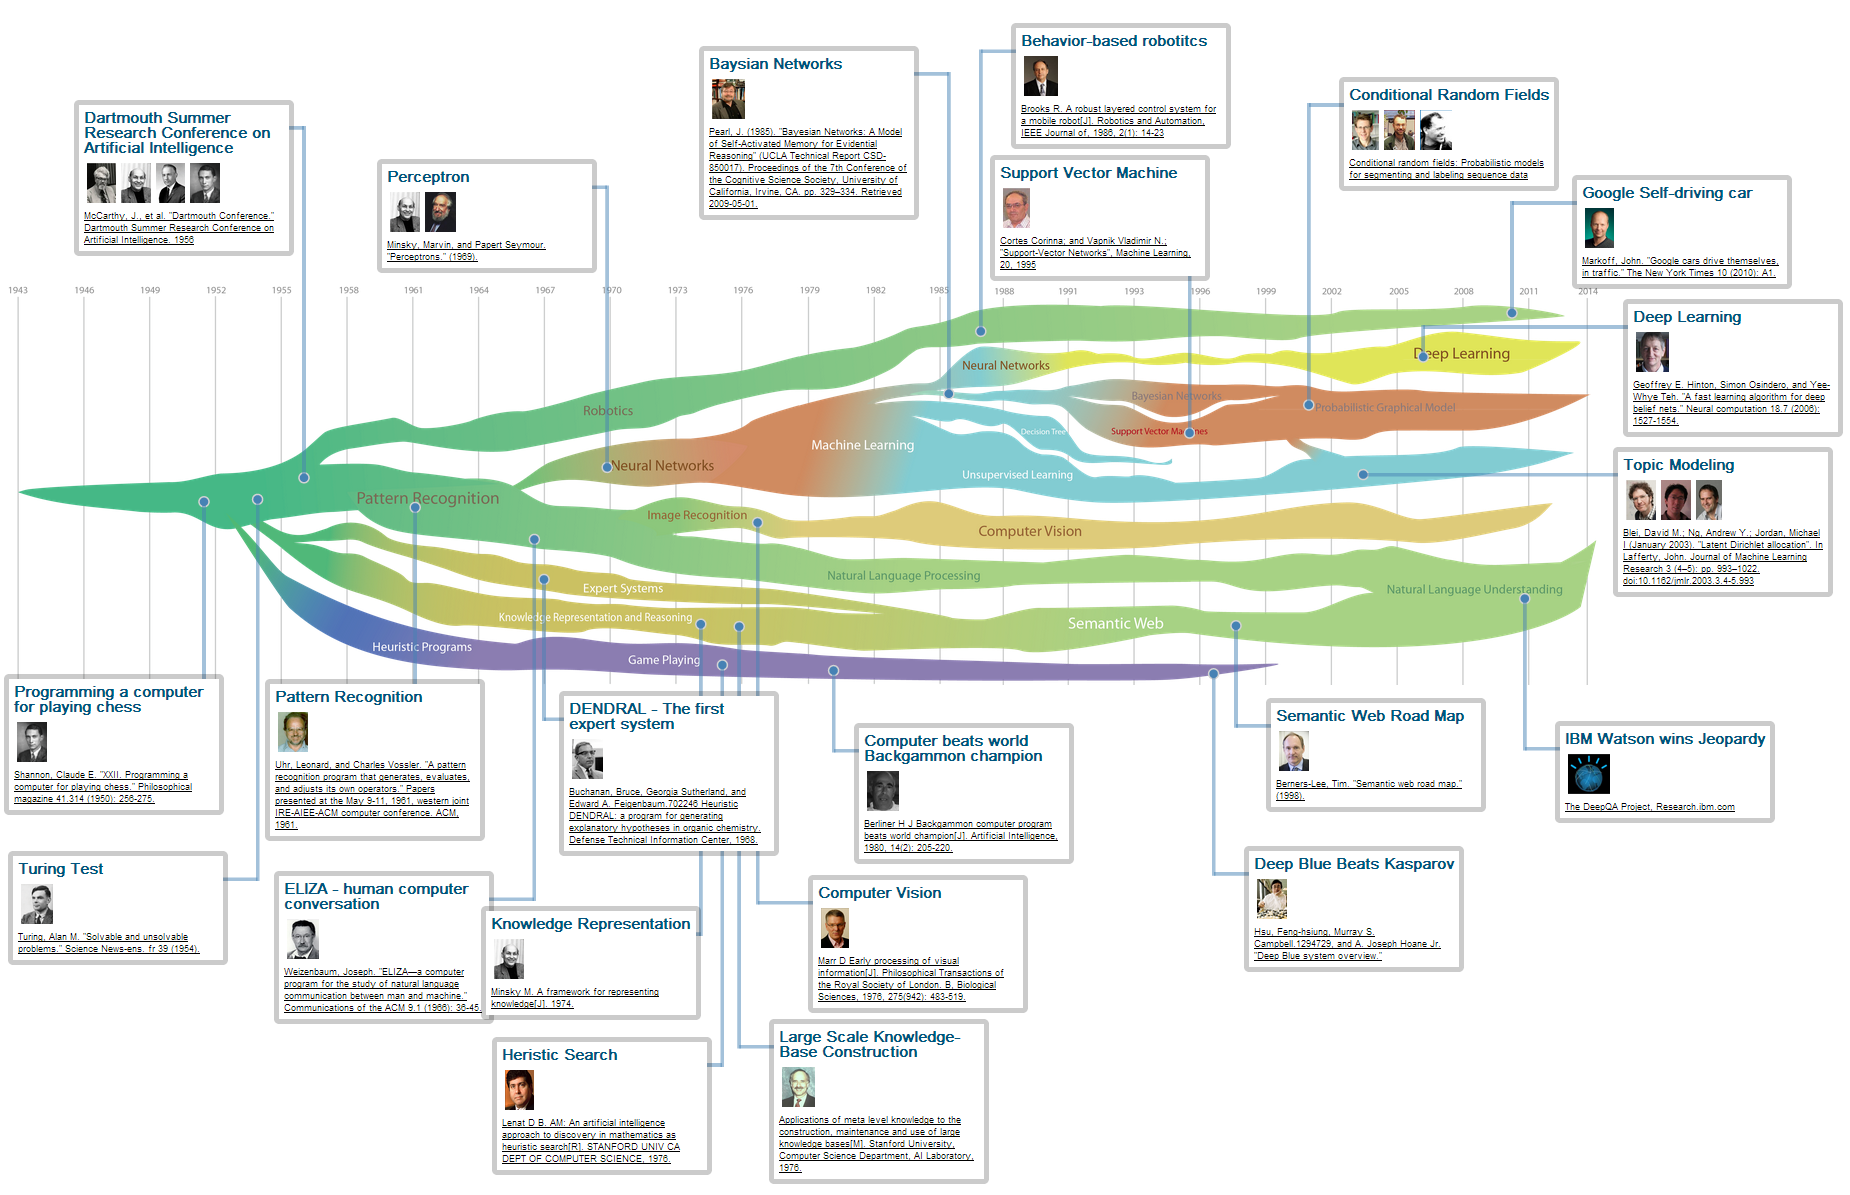
\includegraphics[angle=0,width=0.95\linewidth]{images/ai.png}
\\[1em]
   
The evolutionary trend of Artificial Intelligence.
   
}
%%%%%%%%%%%%%%%%%%%%%%%%%%%%%%%%%%%%%%%%%%%%%%%%%%%%%%%%%%%%%%%%%%%%%%%%%%%%%%
  \headerbox{Problem}{name=problem,column=0,row=0}{
%%%%%%%%%%%%%%%%%%%%%%%%%%%%%%%%%%%%%%%%%%%%%%%%%%%%%%%%%%%%%%%%%%%%%%%%%%%%%%
  The goal of this work is to produce intuitive summarizations of given evolving research topics. Extracting knowledge concepts, milestones and the backbone of the evolutionary trend. It is essentially a multi-document summarization problem in a dynamic setting. We need to find clusters of knowledge concepts, researchers and publications that are highly indicative of major research topics.
   
  We choose an optimal summarization of the knowledge evolutionary trend base on \emph{content coverage} and \emph{ burstiness} of words, the method yields intuitive coarse-level summarization of the temporal dynamics of a given research topic.
 }

%%%%%%%%%%%%%%%%%%%%%%%%%%%%%%%%%%%%%%%%%%%%%%%%%%%%%%%%%%%%%%%%%%%%%%%%%%%%%%
  \headerbox{Challenges}{name=contribution,column=0,below=problem}{
%%%%%%%%%%%%%%%%%%%%%%%%%%%%%%%%%%%%%%%%%%%%%%%%%%%%%%%%%%%%%%%%%%%%%%%%%%%%%%
The temporal summarization task consists a set of unique challenges:
  \begin{itemize}
  \item The research topics are not mutually exclusive. The summarization must consist no only the query it self, but also the related topics.
  \item To summarize a research topic, we need to find a meaningful description of the topic. However the definition of "meaningfulness" is subjective.
  \item The arbitrariness of a user given query. Users may want to query unpopular or fine-grained research area which might lead to data sparsity.
  \item The trade off between conciseness and content coverage of the summarization.
  \end{itemize}
  
  }


%%%%%%%%%%%%%%%%%%%%%%%%%%%%%%%%%%%%%%%%%%%%%%%%%%%%%%%%%%%%%%%%%%%%%%%%%%%%%%
\headerbox{Representation}{name=representation,column=2,below=results}{
%%%%%%%%%%%%%%%%%%%%%%%%%%%%%%%%%%%%%%%%%%%%%%%%%%%%%%%%%%%%%%%%%%%%%%%%%%%%%%
We represent the temporal dynamics of knowledge concepts in a dynamic mutual information graph. For each time slide, we create a node for each related knowledge concepts.

\centering{{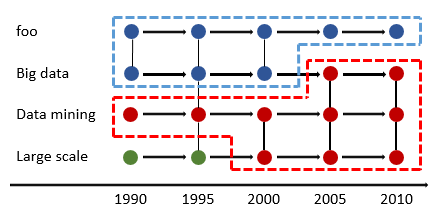
\includegraphics[width=0.98\linewidth]{images/mutual.png}}}
\\[1em]
	There are two types of edges in the graph:
  	\begin{itemize}	
  	\item The concepts in the same time slide are connected with mutual info edge. For an arbitrary edge $(u, v)$, the influence probability from $u$ to $v$ is $P(u,v) = \frac{I(u,v)}{I(u,u)}$, where $I(u,v)$ indicates the mutual information between $u$ and $v$.
	\item Nodes corresponding to the same knowledge concept within two adjacent time slides are connected by an evolving edge, indicates the knowledge concept is evolved from itself in the last time slide. The weight of the evolving edge is a parameter controlling the temporal smoothness of the summarization.
	\end{itemize}
}

%%%%%%%%%%%%%%%%%%%%%%%%%%%%%%%%%%%%%%%%%%%%%%%%%%%%%%%%%%%%%%%%%%%%%%%%%%%%%%
  \headerbox{References}{name=references,column=0,above=bottom}{
%%%%%%%%%%%%%%%%%%%%%%%%%%%%%%%%%%%%%%%%%%%%%%%%%%%%%%%%%%%%%%%%%%%%%%%%%%%%%%
    \smaller
    \bibliographystyle{ieee}
    \renewcommand{\section}[2]{\vskip 0.05em}
    
    \begin{thebibliography}{4}\itemsep=-0.01em
    \setlength{\baselineskip}{0.4em}
    \bibitem{amberg11:bnb}
      Chi Wang, Xiao Yu, Yanen Li, Chengxiang Zhai, and Jiawei Han
      \newblock Content Coverage Maximization on Word Networks for Hierarchical Topic Summarization.
      \newblock In {\em CIKM '13}
		
 \vspace{0.5em}
      \setlength{\baselineskip}{0.4em}
      \bibitem{Chieu:2004:QBE:1008992.1009065}
        Chieu, Hai Leong and Lee, Yoong Keok
        \newblock Query Based Event Extraction Along a Timeline
        \newblock In {\em SIGIR '04}
 \vspace{0.5em}
    \setlength{\baselineskip}{0.4em}
    \bibitem{amberg11:bnb}
      Cui, Weiwei, Shixia Liu, Li Tan, Conglei Shi, Yangqiu Song, Zekai Gao, Huamin Qu, and Xin Tong. 
      \newblock Textflow: Towards better understanding of evolving topics in text.
      \newblock In {\em Visualization and Computer Graphics, IEEE Transactions on 17, no. 12 (2011): 2412-2421.}
 \vspace{0.5em}

    \setlength{\baselineskip}{0.4em}
    \bibitem{amberg11:bnb}
    Griffiths, T., M. Jordan, J. Tenenbaum, and David M. Blei. 
      \newblock Hierarchical topic models and the nested Chinese restaurant process.
      \newblock In {\em Advances in neural information processing systems 16 (2004): 106-114.}
    \end{thebibliography}
 

   \vspace{0.3em}
  }
%%%%%%%%%%%%%%%%%%%%%%%%%%%%%%%%%%%%%%%%%%%%%%%%%%%%%%%%%%%%%%%%%%%%%%%%%%%%%%
  \headerbox{Online Demo}{name=demo,column=2,above=bottom}{
%%%%%%%%%%%%%%%%%%%%%%%%%%%%%%%%%%%%%%%%%%%%%%%%%%%%%%%%%%%%%%%%%%%%%%%%%%%%%%
  \noindent
  \begin{minipage}{\linewidth}
  \begin{minipage}{0.95\linewidth}
    \indent{}The online demo is available at \\
    \url{http://arnetminer.org/event/aihistory}
  \end{minipage}\hfill%
  %\begin{minipage}{0.23\linewidth}
  %\hfill
\includegraphics[width=\linewidth]{chart}
  %\end{minipage}
  \end{minipage}
  }
%%%%%%%%%%%%%%%%%%%%%%%%%%%%%%%%%%%%%%%%%%%%%%%%%%%%%%%%%%%%%%%%%%%%%%%%%%%%%%
  \headerbox{Wisdom of The Crowd}{name=formulation,column=0,below=contribution,above=references}{
%%%%%%%%%%%%%%%%%%%%%%%%%%%%%%%%%%%%%%%%%%%%%%%%%%%%%%%%%%%%%%%%%%%%%%%%%%%%%%
%We use a \emph{information-centric} approach to interpret the summarization quality.
	We will leverage user interactions to involve human into the loop. The system will captures the revisions provided by the users and use them to further refine the summarization result.

}
 
%%%%%%%%%%%%%%%%%%%%%%%%%%%%%%%%%%%%%%%%%%%%%%%%%%%%%%%%%%%%%%%%%%%%%%%%%%%%%%
  %\begin{environment-name}

  %\end{environment-name}\headerbox{Wisdom of The Crowd}{name=strategy,column=1,above=bottom}{
%%%%%%%%%%%%%%%%%%%%%%%%%%%%%%%%%%%%%%%%%%%%%%%%%%%%%%%%%%%%%%%%%%%%%%%%%%%%%%
	%We will leverage user interactions to further refine the summarization result.
  %}
%%%%%%%%%%%%%%%%%%%%%%%%%%%%%%%%%%%%%%%%%%%%%%%%%%%%%%%%%%%%%%%%%%%%%%%%%%%%%%
\headerbox{Method}{name=solution,column=1,row=0,below=results}{
  %%%%%%%%%%%%%%%%%%%%%%%%%%%%%%%%%%%%%%%%%%%%%%%%%%%%%%%%%%%%%%%%%%%%%%%%%%%%%%
We introduce a community-based summarization as we first find a core community (a group of experts) around the topic, and then aggregate each member's research work as the research area. To avoid some authoritative experts dominates the research area and introduce bias, we normalize each member's contribution averagely.
  
With the retrieved document collection, we extract the knowledge concepts mentioned in each documents and construct a dynamic mutual information graph. The following task is to choose a set of high level concepts best summarize the whole research area. We use two measures: \emph{Coverage} and \emph{Burstiness} to choose the concepts of interest.




We use a influence maximization based model to model information coverage of knowledge concepts. Formally we choose a set of $k$ concepts that maximize the content coverage. Meanwhile, we model burstiness by assuming the arrival of words as a unknown binomial distribution, and use $\chi^2$ tests to check for significant association between word and time periods. We calculate the contingency table as following and $\chi^2 = \frac{(ad-bc)^2n}{(a+b)(c+d)(a+c)(b+d)}$.
\begin{center}
\begin{tabularx}{0.5\textwidth}{ |X|X|X| }
  \hline
  - & $W$ & $\bar{W}$ \\
  \hline
  $t$  & a  & b  \\
  \hline
  $<t$  & c  & d  \\
  \hline
\end{tabularx}
\end{center}

After choosing a set of summarization words, we further grouping the rest of the words into clusters, and finally we can use the clusters over time to indict evolving trend and generates the highly intuitive visualization.

}

\end{poster}

\end{document}

